\documentclass{article}

\usepackage[utf8]{inputenc}
\usepackage{graphicx} 
\usepackage{float}
\usepackage{geometry}
\geometry{left=2cm, right=2cm, top=2cm ,bottom=2cm}
\usepackage{amsmath}
\usepackage{textcomp}
\usepackage{tabularx}
\usepackage{url}
\usepackage{hyperref}
\title{Implementation of an On-Grid Solar PV System with Integrated Battery Backup for a Standard Residential Home}
\author{Saad Hajjih}
\date{May 2025}

\begin{document}

\maketitle
\tableofcontents
\listoffigures
\listoftables

\newpage
\begin{abstract}
This paper presents the design, implementation, and analysis of an on-grid solar photovoltaic (PV) system with integrated battery backup tailored for a standard residential home in Amman, Jordan. The proposed system is engineered to meet a daily energy demand of 36 kWh using a PV array rated at 8.28 kW and a lithium-ion battery bank providing 73.7 kWh of usable energy. A hybrid inverter ensures seamless integration between PV generation, storage, and the utility grid. A MATLAB-based simulation over 30 days, including a full-day grid outage, demonstrates the system's autonomy, efficiency, and reliability. A detailed cost analysis validates the feasibility of the solution.
\end{abstract}

\section{Load Profile and Site Conditions}
The residential site at coordinates 31.9951389°N, 35.9400000°E has an average daily energy consumption of 36 kWh and a peak demand of 6.5 kW. Solar resource data from NASA and the Global Solar Atlas show an average peak sun hour (PSH) of 5.891. The optimal fixed tilt angle for maximum energy yield is 29°, with seasonal adjustments of 47° in winter, 32° in spring/fall, and 17° in summer.

\section{System Sizing}
\begin{table}[H]
\centering
\begin{tabular}{|c|c|c|c|}
\hline
A1 & Inverter efficiency & 97.6 & Percent (\%) \\
\hline
A2 & Battery Bus voltage & 48 & Voltage (V) \\
\hline
A3 & Inverter AC voltage & 220 & Voltage (V) \\
\hline
A4 & Daily energy consumption & 36 & kWh/day \\
\hline
A5 & Maximum AC power requirement & 6.5 & kW \\
\hline
A6 & Monthly avg energy consumption & 1080 & kWh/month \\
\hline
A7 & Peak Sun Hours & 5.891 & Hours (h) \\
\hline
A8 & Total amp-hour demand per day & 703.125 & Amp-hours (Ah) \\
\hline
B1 & Days of storage desired (autonomy) & 2 & Days \\
\hline
B2 & Allowable depth of discharge limit & 0.9 & (decimal) \\
\hline
B3 & Required battery capacity & 1562.5 & Amp-hours (Ah) \\
\hline
B4 & Amp-hour capacity for selected batteries & 100 & Amp-hours (Ah) \\
\hline
B5 & Number of batteries in parallel & 16 & --- \\
\hline
B6 & Number of batteries in series & 1 & --- \\
\hline
B7 & Total number of batteries & 16 & --- \\
\hline
B8 & Total battery amp-hour capacity & 1600 & Amp-hours (Ah) \\
\hline
C1 & Total energy demand per day & 36 & kWh/day \\
\hline
C2 & Battery round trip efficiency & 0.85 & (decimal) \\
\hline
C3 & Required array output per day & 42.35 & kWh/day \\
\hline
C4 & PV module max power voltage (STC) & 41.5 & Voltage (V) \\
\hline
C5 & PV module guaranteed power output (STC) & 460 & Watts (W) \\
\hline
C6 & Peak sun hours at design tilt & 5.891 & Hours (h) \\
\hline
C7 & Energy output per module per day & 2710 & Watt-hours (Wh) \\
\hline
C8 & Module energy output at operating temp & 2439 & Watt-hours (Wh) \\
\hline
C9 & Modules required to meet energy requirements & 18 & --- \\
\hline
C10 & Modules per string (rounded up) & 6 & --- \\
\hline
C11 & Strings in parallel (rounded up) & 3 & --- \\
\hline
C12 & Total modules to be purchased & 18 & --- \\
\hline
C13 & Nominal rated PV module output & 460 & Watts (W) \\
\hline
C14 & Nominal rated array output & 8280 & Watts (W) \\
\hline
\end{tabular}
\caption{System Design Parameters and Component Sizing}
\label{tab:placeholder}
\end{table}
\newpage
\subsection{PV Array and Battery Sizing}
The design includes 18 Canadian Solar CS3W-460MS modules, each rated at 460 W, yielding a total array capacity of 8.28 kW. The daily energy requirement, accounting for system losses and battery efficiency, necessitates approximately 42.35 kWh/day of PV output. A lithium-ion battery bank comprising 16 SE-G5.1 Pro-B batteries provides 81.92 kWh of nominal capacity and 73.73 kWh of usable energy (90\% DoD). The system is designed for 2-day autonomy.

\subsection{Inverter and Charge Controller}
The Deye 7.6K-SG01LP1 hybrid inverter supports a peak load of 6.5 kW and includes dual MPPTs for optimal solar harvesting. It accepts up to 10.4 kW of PV input and interfaces with 48 V battery banks. Features such as built-in MPPT charge control, smart battery management, and Wi-Fi monitoring enhance system functionality.

\subsection{Cable Sizing}
Cables are sized based on voltage drop calculations. After applying the formulas and assuming cable lengths:

\begin{table}[H]
    \small % optional smaller font for better fit
    \centering
    \begin{tabularx}{\textwidth}{|X|c|c|c|c|c|c|}
    \hline
    Section & Current (A) & Voltage (V) & Length (m) & Voltage Drop (V) & Formula Result & Recommended Cable Size \\
    \hline
    PV Modules $\to$ Battery Bank   & 127.3  & 48   & 10  & 1.92 & $\approx 11.45\, \text{mm}^2$ & 16 mm² \\
    \hline
    Battery Bank $\to$ Inverter     & 150.5  & 48   & 3   & 1.92 & $\approx 8.1\, \text{mm}^2$   & 16--25 mm² \\
    \hline
    Inverter $\to$ AC Load          & 29.55  & 220  & 10  & 8.8  & $\approx 1.16\, \text{mm}^2$  & 4--6 mm² \\
    \hline
    \end{tabularx}
\caption{Cable Sizing and Voltage Drop Calculations for System Connections}
\label{tab:voltage_drop}
\end{table}
\section{protection and auxiliary equipment}
\begin{table}[H]
    \small
    \centering
    \begin{tabularx}{\textwidth}{|X|X|X|}
    \hline
    Protection Point & Device Type & Rating / Action \\
    \hline
    PV Array $\to$ Inverter (DC) & DC-rated breakers or PV-specific fuses & 16 A per string \\
    \hline
    Battery $\to$ Inverter & DC-rated MCCB or battery fuses & 250 A \\
    \hline
    Inverter $\to$ AC Load & Standard AC breakers & 40 A \\
    \hline
    \end{tabularx}
    \caption{Electrical Protection Devices and Ratings for System Safety}
    \label{tab:protection_devices}
\end{table}
Protection devices are essential for ensuring system safety and reliability. Each PV string is protected with DC-rated breakers or PV fuses rated at 16 A, while the battery-to-inverter connection uses a 250 A DC-rated MCCB or fuse to manage high current levels. On the AC side, a 40 A breaker protects the inverter output to the load. These devices are typically installed in combiner boxes, which may also include additional protection components such as surge protection devices (SPDs), and IP68-rated enclosures, providing full protection against dust ingress and prolonged water immersion.
\subsection{Types of Combiner Boxes}
Combiner boxes come in various types, each designed to cater to specific solar panel installation requirements. Understanding the different types can help you choose the right one for your PV system:
\subsubsection{Standard Combiner Boxes: }
These are the most common type, designed to combine multiple DC inputs from a solar array into a single output. They are ideal for standard solar installations where simplicity and efficiency are key.
\subsubsection{Disconnect Combiner Boxes: }
These boxes offer the added functionality of disconnecting the solar array at a single point. This feature provides an extra layer of safety, allowing for quick and easy shutdowns during emergencies or maintenance.
\subsubsection{AFCI Combiner Boxes: }
Arc Fault Circuit Interrupter (AFCI) combiner boxes are designed to detect arc fault signals and interrupt the circuit before faults can develop into fires or short circuits. This makes them an excellent choice for installations where fire safety is a primary concern. In some areas AFCI combiner boxes are a requirement according to code standards in certain jurisdictions, although this is more relevant for residential installations as opposed to utility-scale solar plants.
\subsubsection{AC Combiner Boxes: }
These boxes are equipped with an integrated AC Molded Case Circuit Breaker (MCCB) for AC input. They are generally used for applications like aggregating AC circuits from inverters in larger systems or handling multiple inverters. They also include Type 2 AC Surge Protection Devices (SPD) for overvoltage protection on inverters, making them suitable for systems that require robust AC protection.\bigskip

   For this system, a Voltacon 9-in/1-out solar PV combiner box is selected, featuring integrated DC fuses, surge protection devices (SPDs), and a DC isolator. It aggregates power from nine PV strings, each comprising two 460 W modules, into a single, protected DC output for the inverter. Each string is individually protected with 16 A fuses to guard against overcurrent, while the integrated SPD offers defense against voltage surges from lightning or grid anomalies. The built-in DC isolator enables safe shutdown and maintenance of the PV array. Housed in a durable, IP65-rated enclosure, the combiner box is well-suited for outdoor installation in demanding environmental conditions. 
   \section{simulation, performance and cost analysis}
   \subsection{System Overview}
\begin{table}[H]
    \small
    \centering
    \begin{tabularx}{\textwidth}{|X|X|}
    \hline
    \textbf{Component} & \textbf{Value} \\
    \hline
    Simulation Duration & 30 Days (May 2025) \\
    \hline
    Daily Load Demand & 36 kWh \\
    \hline
    Total Load (Month) & 1,080 kWh \\
    \hline
    PV Daily Production & 42.35 kWh \\
    \hline
    Total PV Energy & $\sim$1,270.5 kWh \\
    \hline
    Battery Capacity & 1600 Ah @ 48 V = 76.8 kWh \\
    \hline
    Usable Battery (90\% DoD) & 69.12 kWh \\
    \hline
    Inverter Efficiency & 97.6\% \\
    \hline
    Battery Efficiency & 85\% (round-trip) \\
    \hline
    \end{tabularx}
    \caption{Simulation and System Parameters}
    \label{tab:sim_system_params}
\end{table}
\subsection{ single line diagram}
  \begin{figure}[h]
      \centering
      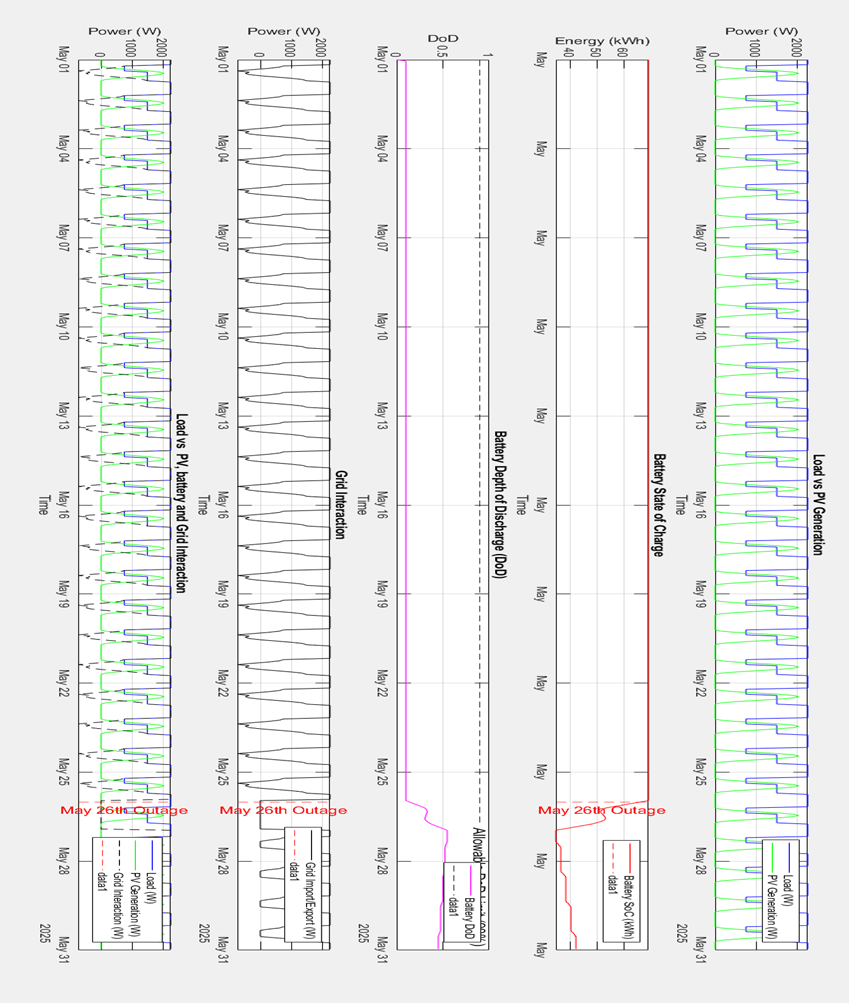
\includegraphics[ width=0.7\linewidth]{figures/Picture1.png}
      \caption{Integrated Solar PV System with Inverter, Battery Bank, and Grid Connection }
      \label{fig:placeholder}
  \end{figure}
\subsection{Performance Analysis}
\begin{figure}[H]
    \centering
    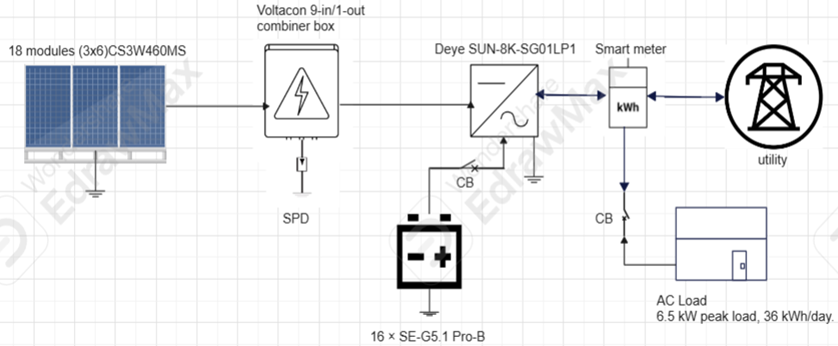
\includegraphics[width=1.\linewidth]{figures/Picture2.png}
    \caption{System Performance Simulation using MATLAB}
    \label{fig:placeholder}
\end{figure}
\subsubsection{Load vs PV Generation}
Most days, photovoltaic production matches the demand closely. On average, photovoltaic energy generates approximately 6.35 kWh/day more than is consumed, allowing potential export to the grid or additional battery charging.
\newpage
\subsubsection{Battery State of Charge (Soc)}
On normal days, the battery remains near full capacity as a result of a consistent surplus of photovoltaic energy.
During the 26 May outage, the state of charge (SoC) drops significantly, confirming the system's dependence on the battery; however, it maintains energy without full depletion.
\subsubsection{Depth of Discharge (DoD)}
During the outage, the Depth of Discharge (DoD) remains safely below 90\% , preserving battery health and ensuring system reliability. Although some energy is lost during the charging and discharging process due to the battery's 85\%  round-trip efficiency, these losses do not affect the overall operation of the system.
\subsubsection{Grid Interaction}
During normal days, excess solar energy is exported to the grid during midday hours, while grid imports typically occur at night to meet the load. In the outage period, the system operates without any grid interaction, and the battery seamlessly supplies the entire load, demonstrating its effectiveness and autonomy.
\subsubsection{Combined View}
On 26 May , during the simulated outage event, the combined output from the PV system and battery successfully met the load demand. Although the battery experienced significant discharge, it did not fully deplete, indicating that the system is appropriately sized for such contingencies.
\subsection{Cost Analysis }
The solar PV system is designed with 16 SE-G5.1 Pro-B lithium batteries and 18 CS3W-460MS solar panels. The total equipment cost, including batteries, PV modules, combiner box, and inverter, is approximately 31255 JD. Adding installation and miscellaneous expenses estimated at 20\% of equipment cost (about 6251 JD), the total system cost comes to roughly 37506 JD. This budget covers all major components and installation for a reliable 2-day autonomy solar energy system.
\begin{table}[H]
    \centering
    \begin{tabular}{|l|c|c|c|}
    \hline
    \textbf{Component} & \textbf{Unit Cost (JD)} & \textbf{Qty} & \textbf{Subtotal (JD)} \\
    \hline
    SE-G5.1 Pro-B Battery (5.12 kWh) & 1,560.00 & 16 & 24,960.00 \\
    CS3W-460MS PV Panels (460W)      & 257.85   & 18 & 4,641.16 \\
    Combiner Box (Voltacon)          & –        & 1  & 391.91 \\
    Inverter (SUN-8K-SG01LP1)        & –        & 1  & 1,262.02 \\
    \hline
    \textbf{Total Equipment}         &          &    & \textbf{31,255.09} \\
    Installation \& Misc. (20\%)     & –        & –  & 6,251.00 \\
    \hline
    \textbf{Total System Cost}       &          &    & \textbf{37,506.09 JD} \\
    \hline
    \end{tabular}
    \caption{Cost Breakdown of System Components and Installation}
    \label{tab:cost_breakdown}
\end{table}
\section{ Conclusion}
In this project, I designed and simulated an on-grid solar PV system with battery storage for a typical residential home with a daily energy consumption of 36 kWh. Using MATLAB, I modeled the system for a full month (May 2025) and included a full-day grid outage on May 26 to test the system’s autonomy and reliability.
The setup includes 18 solar panels producing about 42.35 kWh/day and a battery bank of 16 SE-G5.1 Pro-B lithium-ion batteries. These batteries offer a total of around 81.92 kWh of storage at 48V, with about 73.73 kWh usable, considering a 90\% depth of discharge . During the grid outage simulation, the batteries handled the entire load without going below the DoD limit, proving that the system is well-sized and reliable for backup scenarios.
From a cost perspective, the full system — including panels, batteries, inverter, combiner box, and installation — comes to roughly 37,506 JD. I made sure to select components that are efficient and compatible, like the Deye SUN-8K hybrid inverter and Voltacon combiner box, which helped optimize performance and safety.
Overall, the results showed that the system can easily meet daily energy demands, cover short-term outages, and even export surplus energy on normal days. 
\bibliographystyle{plain}
\bibliography{References}  % Replace with your .bib file name (no .bib extension)
\nocite{*}
\end{document}
